%\documentclass[english]{beamer}
\documentclass[english,hangout]{beamer}
%\documentclass[aspectratio=169]{beamer}
%\usepackage{amsmath}
%\usepackage{amssymb}
\usepackage{rotating}
\usepackage{verbatim}
\usepackage{latexsym}
\usepackage{graphicx}
\usepackage{tabularx}
\usepackage{ragged2e}
\usepackage{eurosym}   % Euro symbol: \euro
\usepackage{listings}
\usepackage{multirow}
\usepackage{colortbl}
\usepackage{textcomp}  % many special symbols
\usepackage{lmodern}
\usepackage{times}
\usepackage[T1]{fontenc}
\usepackage[utf8]{inputenc}
\usepackage[english]{babel}
\usepackage{booktabs}

\colorlet{punct}{red!60!black}
\definecolor{background}{HTML}{EEEEEE}
\definecolor{delim}{RGB}{20,105,176}
\colorlet{numb}{magenta!60!black}

\lstdefinelanguage{json}{
    basicstyle=\normalfont\ttfamily,
    numbers=left,
    numberstyle=\scriptsize,
    stepnumber=1,
    numbersep=8pt,
    showstringspaces=false,
    breaklines=true,
    frame=lines,
    backgroundcolor=\color{background},
    literate=
     *{0}{{{\color{numb}0}}}{1}
      {1}{{{\color{numb}1}}}{1}
      {2}{{{\color{numb}2}}}{1}
      {3}{{{\color{numb}3}}}{1}
      {4}{{{\color{numb}4}}}{1}
      {5}{{{\color{numb}5}}}{1}
      {6}{{{\color{numb}6}}}{1}
      {7}{{{\color{numb}7}}}{1}
      {8}{{{\color{numb}8}}}{1}
      {9}{{{\color{numb}9}}}{1}
      {:}{{{\color{punct}{:}}}}{1}
      {,}{{{\color{punct}{,}}}}{1}
      {\{}{{{\color{delim}{\{}}}}{1}
      {\}}{{{\color{delim}{\}}}}}{1}
      {[}{{{\color{delim}{[}}}}{1}
      {]}{{{\color{delim}{]}}}}{1},
}

%\usetheme[fb2]{FrankfurtUniversity}
\usetheme[fb2,noslogan]{FrankfurtUniversity}
%\slogan{\large\color{red}UNAUTHORIZED}


\title{Blockchain Solution to\\Healthcare Record System using\\Hyperledger Fabric}
\subtitle{Sprint 3 Review}
\author{Team Lithium}
%\institute{Frankfurt University of Applied Sciences\\}
\date{\today}%{November 24, 2020}


\begin{document}


\begin{frame}
\titlepage
\end{frame}
%\addtocounter{framenumber}{-1}



\begin{frame}
   \frametitle{Agenda}
   \tableofcontents%[hideallsubsections]
\end{frame}




\section{Sprint 3}

\subsection{Results}

\begin{frame}[fragile]
 \frametitle{Sprint 3}
 \framesubtitle{Results - Overview}
  \begin{itemize}
    % TODO: ADD points for sprint 3 result
    \item Development of UI for admin, doctor and patient.
    \item Integration of UI with REST APIs and smartcontracts.
    \item Integration of redis database to store doctor credentials. 
    \item Creation of connection profile for each user like doctor, patients and patients stored in initledger.
    \item Implementation of login/logout for doctor and patient and grant/revoke backend APIs.
    \item Creation of separate APIs/smartcontracts in a chaincode for admin, doctor and patient.
    \item Hash operation is performed on the patient password field and stored to ledger.
  \end{itemize}
\end{frame}

\begin{frame}[fragile]
 \frametitle{Sprint 3}
 \framesubtitle{Results - Overview}
\begin{center}
        \vspace{-1.2em}
            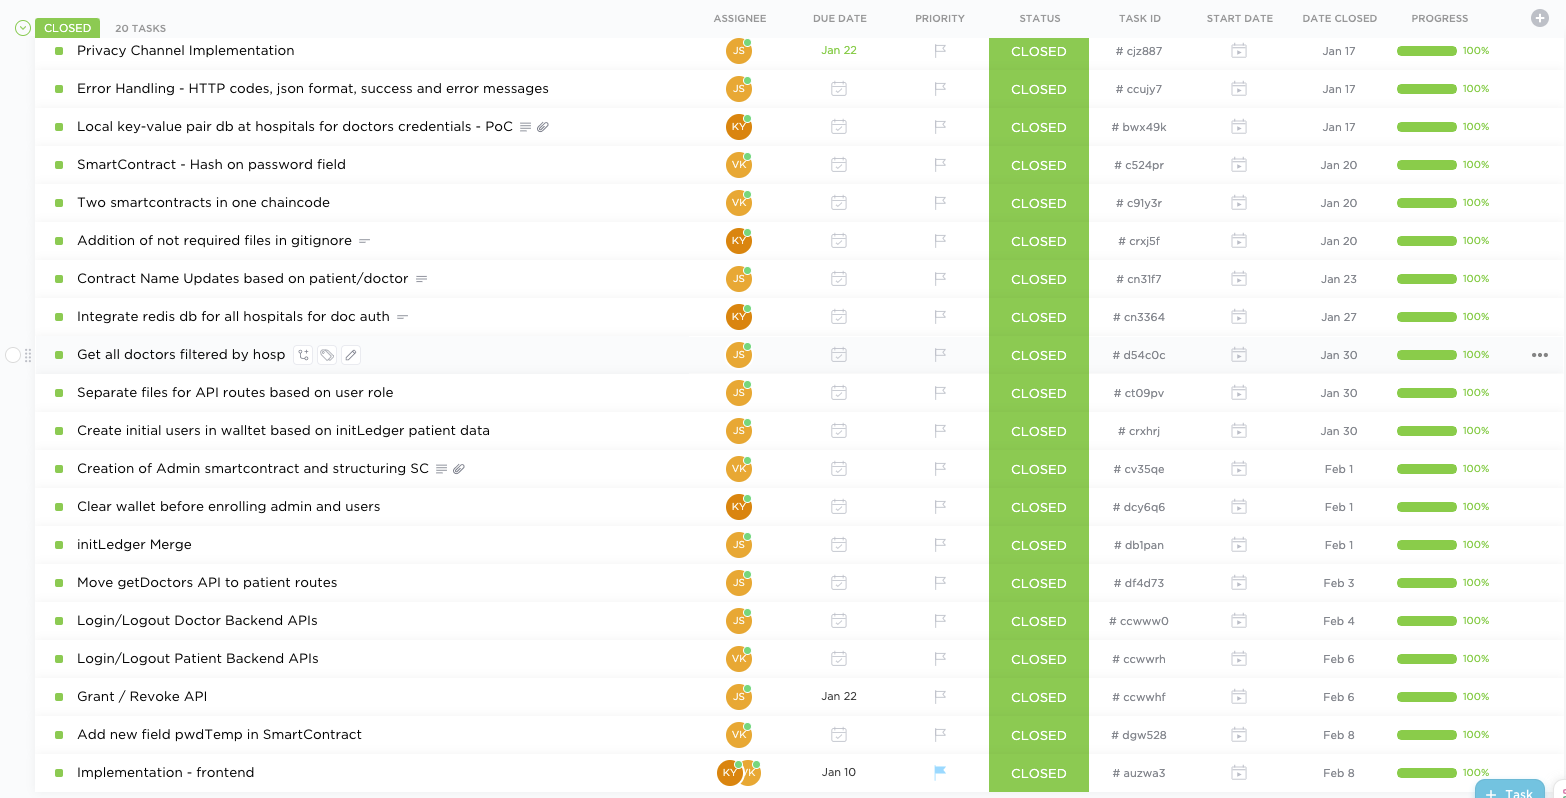
\includegraphics[height=6cm]{Sprint3Result.png}
        \end{center}
\end{frame}

\subsection{Pending Tasks}

\begin{frame}[fragile]
 \frametitle{Sprint 3}
 \framesubtitle{Pending Tasks}
\begin{center}
        \vspace{-1.2em}
            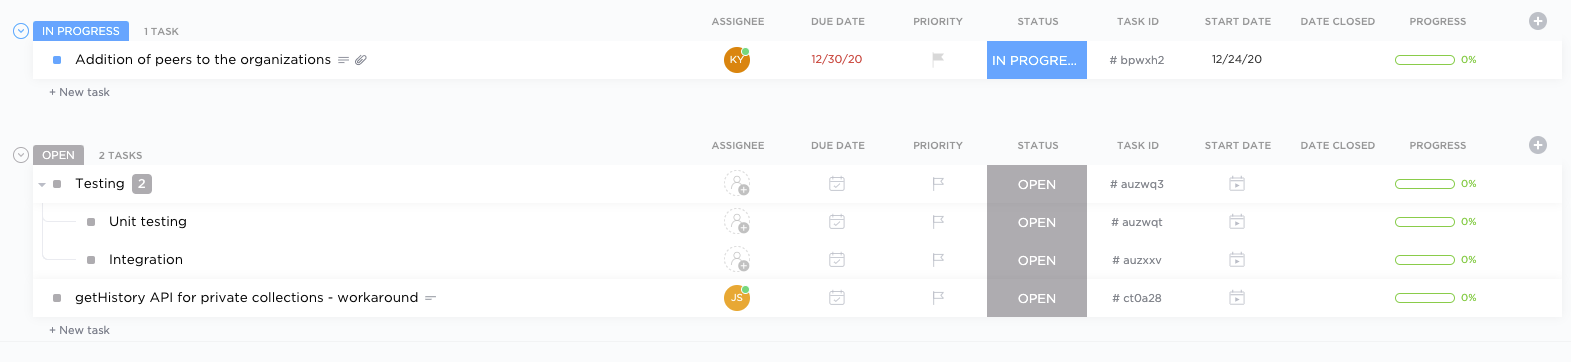
\includegraphics[height=2.7cm]{Sprint3Pendin.png}
        \end{center}
\end{frame}

\subsection{Demo}

\begin{frame}[fragile]
 \frametitle{Sprint 3}
    \begin{center}
        \vspace{-1.2em}
            Demo
        \end{center}
\end{frame}

\section{Sprint 4}

\subsection{Overview}

\begin{frame}[fragile]
 \frametitle{Sprint 4}
 \framesubtitle{Overview}
    \begin{itemize}
        \item Exam break up to March 5th
        \item Daily scrum as usual starting from March 9th 2021
        \item Final project presentation: Screencast
        \item Code freeze on March 16th 2021
    \end{itemize}
\end{frame}

\subsection{Tasks}

\begin{frame}[fragile]
 \frametitle{Sprint 4}
 \framesubtitle{Tasks}
    \begin{center}
        \vspace{-1.2em}
            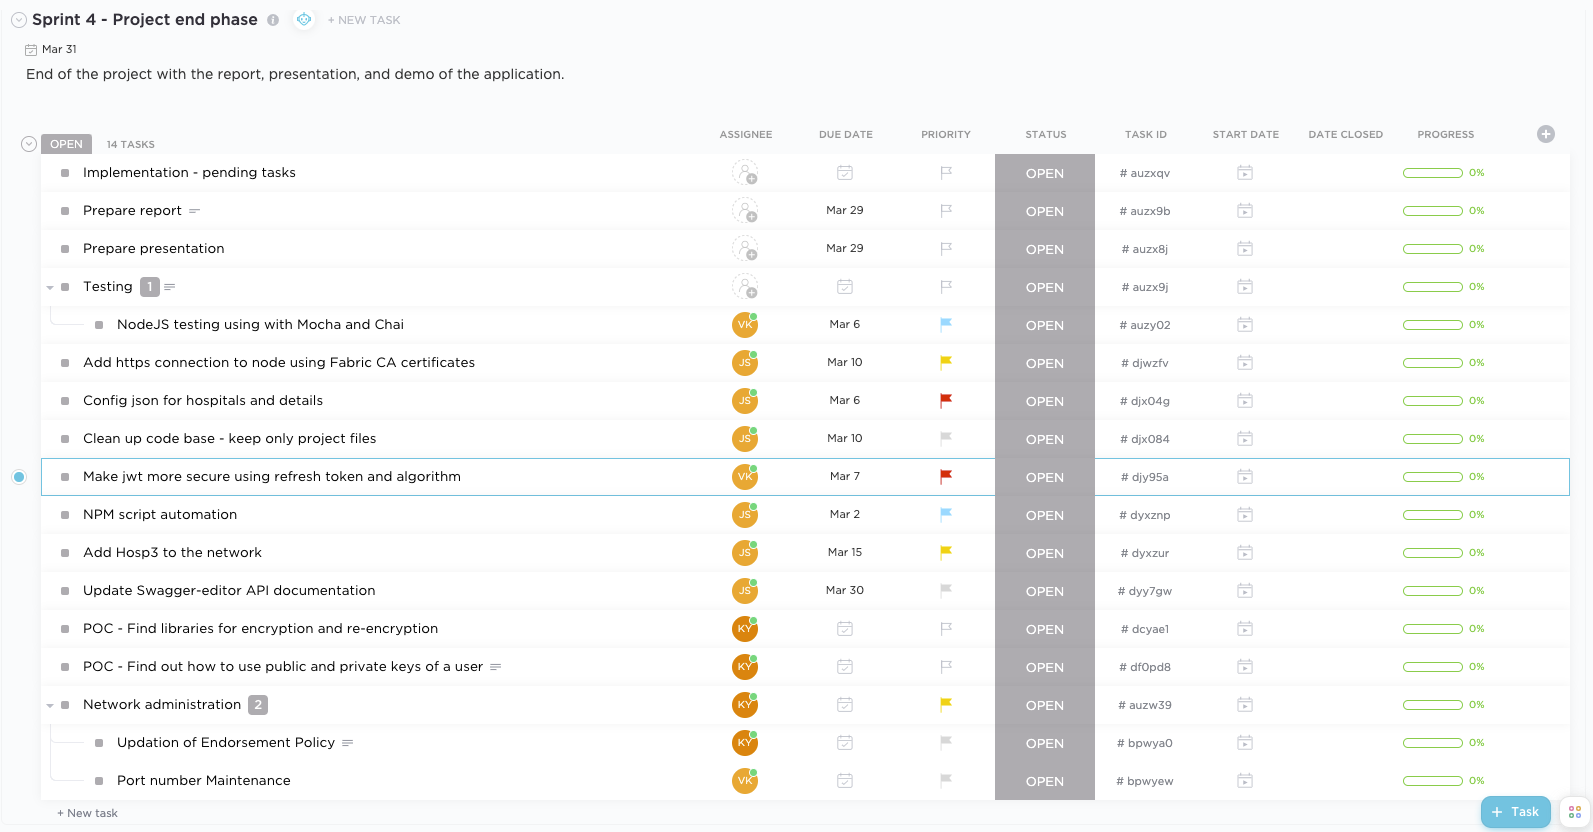
\includegraphics[height=7cm]{Sprint4tasks.png}
    \end{center}
\end{frame}



\section{References}

\begin{frame}
\frametitle{References}
\begin{thebibliography}{00}
\bibitem{b1} https://www.ncbi.nlm.nih.gov/pmc/articles/PMC7010942/
\bibitem{b2} https://www.ncbi.nlm.nih.gov/pmc/articles/PMC7474412/
\bibitem{b3} https://www.sciencedirect.com/science/article/pii/S2214212-619306155
\bibitem{b4} https://hyperledger-fabric.readthedocs.io/ Accessed-On:12/01/2021
\bibitem{b5} https://medium.com/@lichunshen84/build-a-blockchain-poc-application-using-hyperledger-fabric-5a32687072b7, Accessed-On:01/12/2020
\end{thebibliography}

\end{frame}


\end{document}